%%%%%%%%%%%%%%%%%%%%%%%%%%%%%%%%%%%%%%%%%
% a0poster Portrait Poster
% LaTeX Template
% Version 1.0 (22/06/13)
%
% The a0poster class was created by:
% Gerlinde Kettl and Matthias Weiser (tex@kettl.de)
% 
% This template has been downloaded from:
% http://www.LaTeXTemplates.com
%
% License:
% CC BY-NC-SA 3.0 (http://creativecommons.org/licenses/by-nc-sa/3.0/)
%
%%%%%%%%%%%%%%%%%%%%%%%%%%%%%%%%%%%%%%%%%

%----------------------------------------------------------------------------------------
%	PACKAGES AND OTHER DOCUMENT CONFIGURATIONS
%----------------------------------------------------------------------------------------

\documentclass[a0,portrait]{a0poster}

\usepackage{multicol} % This is so we can have multiple columns of text side-by-side
\columnsep=100pt % This is the amount of white space between the columns in the poster
\columnseprule=3pt % This is the thickness of the black line between the columns in the poster

\usepackage[svgnames]{xcolor} % Specify colors by their 'svgnames', for a full list of all colors available see here: http://www.latextemplates.com/svgnames-colors

\usepackage{times} % Use the times font
%\usepackage{palatino} % Uncomment to use the Palatino font

\usepackage{graphicx} % Required for including images
\graphicspath{{../tex/imgs/}} % Location of the graphics files
\usepackage{booktabs} % Top and bottom rules for table
\usepackage[font=small,labelfont=bf]{caption} % Required for specifying captions to tables and figures
\usepackage{amsfonts, amsmath, amsthm, amssymb} % For math fonts, symbols and environments
\usepackage{wrapfig} % Allows wrapping text around tables and figures

% To use subfigure
\usepackage{caption}
\usepackage{subcaption}
\usepackage{algorithm}
\usepackage{algpseudocode}

\newcommand{\spc}{\phantom{a}}

\begin{document}

%----------------------------------------------------------------------------------------
%	POSTER HEADER 
%----------------------------------------------------------------------------------------

% The header is divided into two boxes:
% The first is 75% wide and houses the title, subtitle, names, university/organization and contact information
% The second is 25% wide and houses a logo for your university/organization or a photo of you
% The widths of these boxes can be easily edited to accommodate your content as you see fit

\begin{minipage}[c]{0.70\linewidth}
\veryHuge \color{NavyBlue} \textbf{A shuffled complex evolution algorithm for
the multidimensional knapsack problem} \color{Black} % Title
\end{minipage}
\begin{minipage}[c]{0.30\linewidth}
  %\hspace{0.25\linewidth}
  \hfill
  
\includegraphics[scale=2.5]{ciarp-logo}
\end{minipage}\\[1cm]

\begin{minipage}[c]{0.10\linewidth}
  \vspace{-15mm}
  
\includegraphics[scale=1.5]{../../brasao-ufes}
\end{minipage}
\begin{minipage}[c]{0.80\linewidth}
  \huge \textbf{Marcos Baroni \& Fl\'avio Varej\~ao}\\[0.5cm] % Author(s)
  \huge Universidade Federal do Espírito Santo - Departamento de Inform\'atica\\[0.4cm] % University/organization
  \Large \texttt{marcos.baroni@aluno.ufes.br}\\
\end{minipage}

%\vspace{1cm} % A bit of extra whitespace between the header and poster content

%----------------------------------------------------------------------------------------

\begin{multicols}{2} % This is how many columns your poster will be broken into, a portrait poster is generally split into 2 columns

%----------------------------------------------------------------------------------------
%	ABSTRACT
%----------------------------------------------------------------------------------------

\color{Navy} % Navy color for the abstract

\begin{abstract}

This work addresses the application of
a population based evolutionary algorithm
called shuffled complex evolution (SCE) in the multidimensional knapsack
problem.
The SCE regards a natural evolution happening simultaneously in independent communities.
The performance of the SCE algorithm is verified through computational experiments
using well-known problems from literature and randomly generated problem as well.
The SCE proved to be very effective in finding good solutions demanding a
very small amount of processing time.

{\bf Keywords: } Multidimensional knapsack problem, Meta-heuristics, Artificial Intelligence

\end{abstract}

%----------------------------------------------------------------------------------------
%	INTRODUCTION
%----------------------------------------------------------------------------------------

\color{SaddleBrown} % SaddleBrown color for the introduction

\section*{Introduction}

The multidimensional knapsack problem (MKP) is a strongly NP-hard combinatorial
optimization problem which can be viewed as a resource allocation problem and
defined as follows:

\begin{align*}
  \text{maximize} & \sum_{j=1}^n p_j x_j \\
  \text{subject to} & \sum_{j=1}^n w_{ij} x_j \leqslant c_i \quad i \in \{1, \ldots, m\}\\
   & x_j \in \{0, 1\}, \quad j \in \{1, \ldots, n\}.
\end{align*}

The multidimensional knapsack problem can be applied on budget planning 
scenarios and project selections~\cite{mcmillan1973resource},
cutting stock problems~\cite{Gilmore-Gomory-1966}, loading problems~\cite{Shih-1979},
allocation of processors and databases in distributed computer programs~\cite{Gavish-Pirckul-1982}.

The problem is a generalization of the well-known knapsack problem (KP) in which
$m = 1$.
However it is a NP-hard problem significantly harder to solve in practice than the KP.
Due its simple definition but challenging difficulty of solving, the MKP is often used to
to verify the efficiency of novel metaheuristics.
A good review for the MKP is given by \cite{freville1994efficient}.

In this paper we address the application of a metaheuristic called
shuffled complex evolution (SCE) to the multidimensional knapsack problem.
The SCE is a metaheuristic, proposed by Duan in \cite{duan1992effective},
which combines the ideas of a controlled random search with the concepts
of competitive evolution and shuffling.

\color{DarkSlateGray} % DarkSlateGray color for the rest of the content

\section*{The SCE for the MKP}

\begin{center}
\begin{minipage}{0.30\linewidth}
  \centering
  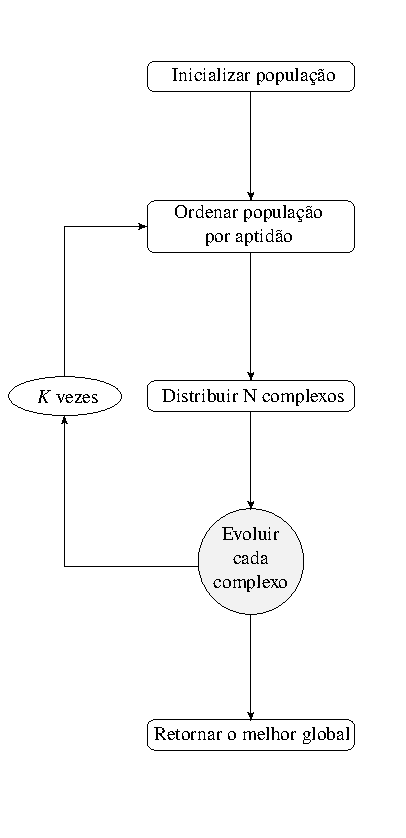
\includegraphics[scale=1.5]{flow1}
  \captionof{figure}{figure caption}
  \label{fig:flow1}
\end{minipage}
\begin{minipage}{0.30\linewidth}
    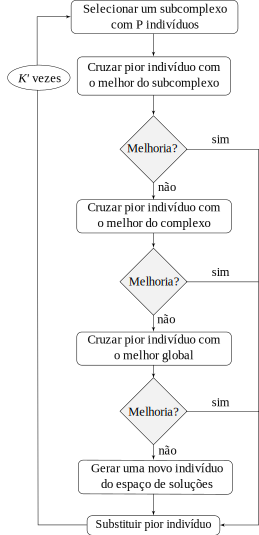
\includegraphics[scale=1.5]{flow2}
  \captionof{figure}{figure caption}
  \label{fig:flow2}
\end{minipage}
\begin{minipage}{0.30\linewidth}
    
\includegraphics[scale=1.5]{alg-new}
	\\[1cm]
    
\includegraphics[scale=1.5]{alg-cross}
  \captionof{figure}{figure caption}
  \label{fig:alg-new}
\end{minipage}
\end{center}

\section*{Computational experiments}




  \begin{tabular}{|c|c|l|}
  \hline
  \multicolumn{1}{|c}{\rule{0pt}{12pt} \spc } & \multicolumn{1}{|c|}{\bf \spc Value \spc } & \multicolumn{1}{c|}{\bf Description} \\[2pt]
  \hline\rule{0pt}{12pt}
  $N$  & $20$  & \spc \# of complexes \\
  $M$  & $20$  & \spc \# of individuals in each complex \\
  $P$  & $5$   & \spc \# of individuals in each subcomplex \\
  $K$  & $300$ & \spc \# of algorithm iterations \\
  $K'$ & $20$  & \spc \# of iterations of evolving process \\
  $c$  & $n/5$ & \spc \# of genes carried from parent in crossing \\[2pt]
  \hline
  \end{tabular}
  \captionof{table}{Parameters used in SCE algorithm.}
  \label{tab:params}



\begin{minipage}[t]{0.5\linewidth}
\hspace{3cm}
\begin{tabular}{|r|r|rr|} \hline
\textbf{n}   & \textbf{m}  & \textbf{SCE t (s)} & \textbf{gap (\%)} \\ \hline
   $100$ & $5$  & $0.81$ & $97.6$ \\
	   & $10$ & $0.86$ & $97.0$ \\
	   & $30$ & $1.02$ & $96.7$ \\ \cline{2-4}
    & \multicolumn{2}{r}{{\bf average gap}}  & $\bf 97.1$  \\ \hline
   $250$ & $5$  & $1.75$ & $95.3$ \\
	   & $10$ & $1.83$ & $95.0$ \\
	   & $30$ & $2.24$ & $94.7$ \\ \cline{2-4}
    & \multicolumn{2}{r}{{\bf average gap}}  & $\bf 95.0$  \\ \hline
   $500$ & $5$  & $3.23$ & $93.7$ \\
	   & $10$ & $3.40$ & $93.7$ \\
	   & $30$ & $3.91$ & $93.3$ \\ \cline{2-4}
    & \multicolumn{2}{r}{{\bf average gap}}  & $\bf 93.6$  \\ \hline
\end{tabular}
 \captionof{table}{SCE performance on Chu-Beasley problems.}
 \label{tab:chu}
\end{minipage}
\begin{minipage}[t]{0.5\linewidth}
\centering
\begin{tabular}[c]{|r|r|r|rrr|} \hline
\textbf{n}   & \textbf{m}  & \textbf{$\alpha$}    &\textbf{SCIP t (s)}& \textbf{SCE t (s)} & \textbf{gap (\%)} \\ \hline
$500$ & $10$ & $0.25$ & $278.85$ & $  2.23$  & $96.1$ \\
    &    & $0.50$ & $177.32$ & $  2.14$  & $98.4$ \\
    &    & $0.75$ & $  8.47$ & $  1.87$  & $99.6$ \\ \cline{2-6}
    & \multicolumn{4}{r}{\textbf{average gap}}  & $\bf 98.0$  \\ \hline
    & $20$ & $0.25$ & $284.11$ & $  2.30$  & $96.7$ \\
    &    & $0.50$ & $275.68$ & $  2.16$  & $98.6$ \\
    &    & $0.75$ & $ 33.67$ & $  1.90$  & $99.7$ \\ \cline{2-6}
    & \multicolumn{4}{r}{\textbf{average gap}}  & $\bf 98.3$  \\ \hline
    & $30$ & $0.25$ & $283.78$ & $  2.50$  & $96.9$ \\
    &    & $0.50$ & $283.54$ & $  2.32$  & $98.7$ \\
    &    & $0.75$ & $ 71.66$ & $  1.96$  & $99.7$ \\ \cline{2-6}
    & \multicolumn{4}{r}{\textbf{average gap}}  & $\bf 98.3$  \\ \hline
\end{tabular}
 \captionof{table}{SCE performance on random generated problems.}
 \label{tab:rand}
\end{minipage}

\color{SaddleBrown} % SaddleBrown color for the conclusions to make them stand out

\section*{Conclusions}

In this work we addressed the application of the shuffled complex
evolution (SCE) to the multidimensional knapsack problem and investigated it
performance through several computational experiments.

The SCE algorithm, which combines the ideas of a controlled random search with
the concepts of competitive evolution proved to be very effective in finding
good solution for hard instances of MKP, demanding a very small amount of
processing time to reach high quality solutions for MKP.

\color{DarkSlateGray} % Set the color back to DarkSlateGray for the rest of the content

%----------------------------------------------------------------------------------------
%	FORTHCOMING RESEARCH
%----------------------------------------------------------------------------------------

\section*{Future remarks}
\begin{itemize}
	\item Application of problem reduction procedures for the MKP;
	\item Investigation of different crossing procedures;
	\item Use of local search in the process of evolving complexes.
\end{itemize}


%\nocite{*} % Print all references regardless of whether they were cited in the poster or not
\bibliographystyle{plain} % Plain referencing style
\bibliography{../../../refs} % Use the example bibliography file sample.bib


\section*{Acknowledgements}
Research supported by Funda\c c\~ao de Amparo \`a Pesquisa do Esp\'irito Santo.

\end{multicols}

\end{document}
